\documentclass[12pt]{article}

%\usepackage{graphics}
\usepackage{graphicx}
\usepackage{caption}
\usepackage{subcaption}
%\usepackage{epsfig}
%\usepackage{times}
%\usepackage{amsmath}
%\usepackage[spanish]{babel}
%\usepackage{lscape}
%\usepackage[nottoc,numbib]{tocbibind}
%\usepackage{pdfpages}

\title{Exercise 2}
\date{\today}
%\author{Mat\'{\i}as Rivero}

\begin{document}
\maketitle

\section{Assignment}
During the design process of a component, the engineer will normally receive as input several design requerimients that the component will have to satisfy. The selection of the apropiate material is one of the major engineering decisions while designing a mechanical component. The usage of adequate constitutive relations in a finite element model allows to simulate very accurately the behaviour of a given material. Under this scenario among others, finite element analysis helps to speed up designing times while reducing costs. 

\medskip

Let's consider a mast which is fixed to the ground and subjected to the wind action. The geometry, material properties and boundary conditions are given by Fig.~\ref{fig:geometry}. The mast can be built using two available materials at the moment: steel or aluminium. Aluminum is cheaper but it is less rigid. The only design condition is that the maximum displacement on $x$ direction can not be larger than $7\,mm$. Will aluminium satisfy the design requeriment?. In case aluminium is not admissible, will steel serve as an alternative?

\begin{itemize}
\item Run this problem using Ostero, assuming geometrical linearity and an elastic material model under plane stress assumption. Postprocess the results with ParaView.
\item Look for the point of maximum $x$ displacement. To do this, split horizontally the Layout and create a SpreadSheet View. You can now sort the displacement values for each nodal point.
\item See if the design requerimient is fulfilled.
\item If not, modify the boundaries file, re-run the case using steel and re-check the condition.
\item Do you think steel would serve as a good substitution?
\end{itemize}

If you get lost, in the RESOLUTION folder you will find several hints that will help you with the fullfilment of this assignment.

\vspace{2cm}

\begin{figure}[htp]
\begin{center}
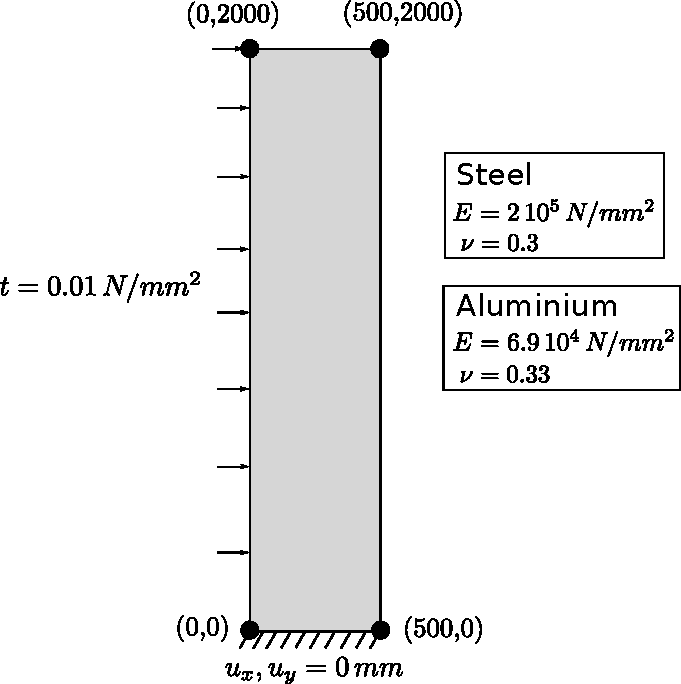
\includegraphics[width=0.6\linewidth]{mast.pdf}
\caption{Geometry, properties and boundary conditions.}
\label{fig:geometry}
\end{center}
\end{figure}

\vspace{2cm}

\hrulefill

%~\cite{bib:belytschko}.
%\begin{thebibliography}{9}
%\bibitem{bib:belytschko} {\it Nonlinear Finite Elements for Continua and Structures}. Ted Belytschko, Wing Kam Liu, Brian Moran. Wiley, 2000. 
%\end{thebibliography}

\end{document}
